\documentclass[aspectratio=43]{beamer}
\usepackage{ragged2e}
\usepackage{multirow}
\usepackage{alltt}

\usetheme{CSCS}
\newcommand{\lst}[1]{\colorbox{white!20!black}{\lstinline!#1!}}
\newcommand{\lstterm}[1]{\colorbox{white}{\lstinline!#1!}}


\newenvironment<>{info}[1]{%
\setbeamercolor{block title}{}%
\begin{tcolorbox}[
colback=white,
colbacktitle=white!85!green,
coltitle=black,
colframe=black,
toptitle=1mm,
bottomtitle=1mm,
lefttitle=3mm,
leftupper=1mm,
leftlower=1mm,
rightupper=1mm,
rightlower=1mm,
boxsep=0mm,
title={#1}]}{\end{tcolorbox}}


\newenvironment<>{terminal}[1]{%
\setbeamercolor{block title}{}%
\begin{tcolorbox}[
colback=white,
colbacktitle=white!85!blue,
colframe=black,
coltitle=black,
toptitle=1mm,
bottomtitle=1mm,
lefttitle=3mm,
leftupper=1mm,
leftlower=1mm,
rightupper=1mm,
rightlower=1mm,
top=-1mm,
bottom=-1mm,
boxsep=0mm,
title={#1}]}{\end{tcolorbox}}

\newenvironment<>{code}[1]{%
\setbeamercolor{block title}{}%
\begin{tcolorbox}[
colback=white!10!black,
colbacktitle=white!85!blue,
colframe=black,
coltitle=black,
toptitle=1mm,
bottomtitle=1mm,
lefttitle=3mm,
leftupper=1mm,
leftlower=1mm,
rightupper=1mm,
rightlower=1mm,
top=-1mm,
bottom=-1mm,
boxsep=0mm,
title={#1}]}{\end{tcolorbox}}

\lstset{
    language=[ANSI]C++,
    showstringspaces=false,
    backgroundcolor=\color{white!10!black},
    basicstyle=\lstfont{white},
    identifierstyle=\lstfont{white},
    keywordstyle=\lstfont{magenta!40!white},
    numberstyle=\lstfont{white},
    stringstyle=\lstfont{cyan},
    commentstyle=\lstfont{yellow!30!white},
    moredelim=[is][\lsttinyfont{green!60!white}]{``}{``},
    emph={
        cudaMalloc, cudaFree,
        cudaDeviceSynchronize,
        cudaMallocHost, cudaFreeHost,
        cudaMallocManaged, cudaMemAttachGlobal,
        cudaMemcpyAsync, cudaMemcpy, cudaMemcpyKind,
        cudaMemcpyHostToDevice, cudaMemcpyDeviceToHost,
        cudaMemcpyHostToHost, cudaMemcpyDeviceToDevice,
        cudaSuccess, cudaGetLastError, cudaGetErrorString,
        cudaErrorMemoryAllocation, cudaError_t,
        cudaOccupancyMaxPotentialBlockSize,
        __global__, __shared__, __device__, __host__,
        __syncthreads,
        cudaEvent_t, cudaStream_t,
        cudaEventCreate, cudaEventSynchronize, cudaEventDestroy,
        cudaEventElapsedTime, cudaEventQuery, cudaEventRecord,
        cudaStreamWaitEvent,
        threadIdx, blockIdx, blockDim, gridDim,
        cudaStream_t, cudaStreamCreate, cudaStreamDestroy,
        dim3,
    },
    emphstyle={\lstfont{green!60!white}},
    breaklines=true
}

\definecolor{codenumber}{rgb}{0.5,0.5,0.5}
\definecolor{codekeyword}{rgb}{0.9,0.4,0.7}
\definecolor{codeCUDA}{rgb}{1.0,0.6,0.6}

\lstdefinestyle{boxcuda}{
    language=[ANSI]C++,
    showstringspaces=false,
    backgroundcolor=\color{white!10!black},
    basicstyle=\lstfont{white},
    identifierstyle=\lstfont{white},
    keywordstyle=\lstfont{magenta!40!white},
    numberstyle=\lstfont{white},
    stringstyle=\lstfont{cyan},
    commentstyle=\lstfont{yellow!30!white},
    moredelim=[is][\lstfont{green!60!white}]{@}{@},
    emph={
        cudaMalloc, cudaFree,
        cudaDeviceSynchronize,
        cudaMallocHost, cudaFreeHost,
        cudaMallocManaged, cudaMemAttachGlobal,
        cudaMemcpyAsync, cudaMemcpy, cudaMemcpyKind,
        cudaMemcpyHostToDevice, cudaMemcpyDeviceToHost,
        cudaMemcpyHostToHost, cudaMemcpyDeviceToDevice,
        cudaSuccess, cudaGetLastError, cudaGetErrorString,
        cudaErrorMemoryAllocation, cudaError_t,
        cudaOccupancyMaxPotentialBlockSize,
        __global__, __shared__, __device__, __host__,
        __syncthreads,
        cudaEvent_t, cudaStream_t,
        cudaEventCreate, cudaEventSynchronize, cudaEventDestroy,
        cudaEventElapsedTime, cudaEventQuery, cudaEventRecord,
        cudaStreamWaitEvent,
        threadIdx, blockIdx, blockDim, gridDim,
        cudaStream_t, cudaStreamCreate, cudaStreamDestroy,
        dim3,
    },
    emphstyle={\lstfont{green!60!white}},
    breaklines=true
}

\lstdefinestyle{boxcudatiny}{
    language=[ANSI]C++,
    showstringspaces=false,
    backgroundcolor=\color{white!10!black},
    basicstyle=\lsttinyfont{white},
    identifierstyle=\lsttinyfont{white},
    keywordstyle=\lsttinyfont{magenta!40!white},
    numberstyle=\lsttinyfont{white},
    stringstyle=\lsttinyfont{cyan},
    commentstyle=\lsttinyfont{yellow!30!white},
    moredelim=[is][\lsttinyfont{green!60!white}]{@}{@},
    emph={
        cudaMalloc, cudaFree,
        cudaDeviceSynchronize,
        cudaMallocHost, cudaFreeHost,
        cudaMallocManaged, cudaMemAttachGlobal,
        cudaMemcpyAsync, cudaMemcpy, cudaMemcpyHostToDevice, cudaMemcpyDeviceToHost,
        cudaSuccess, cudaGetLastError, cudaGetErrorString,
        cudaErrorMemoryAllocation, cudaError_t,
        cudaOccupancyMaxPotentialBlockSize,
        __global__, __shared__, __device__, __host__,
        __syncthreads,
        cudaEvent_t, cudaStream_t,
        cudaEventCreate, cudaEventSynchronize, cudaEventDestroy,
        cudaEventElapsedTime, cudaEventQuery, cudaEventRecord,
        cudaStreamWaitEvent,
        threadIdx, blockIdx, blockDim, gridDim,
        cudaStream_t, cudaStreamCreate, cudaStreamDestroy,
        dim3,
    },
    emphstyle={\lstfont{green!60!white}},
    breaklines=true
}

\lstdefinestyle{terminal}{
    language=bash,
    showstringspaces=false,
    backgroundcolor=\color{white},
    basicstyle=\lsttinyfont{black},
    identifierstyle=\lsttinyfont{black},
    keywordstyle=\lsttinyfont{black},
    numberstyle=\lsttinyfont{black},
    stringstyle=\lsttinyfont{black},
    commentstyle=\lsttinyfont{green!30!black},
    emph={ srun, make, nvcc, salloc, git, ssh },
    emphstyle={\lsttinyfont{blue}},
    breaklines=true
}


\newcommand{\SummerSchoolYear}{2016}
\newcommand{\SummerSchoolDate}{July 20 -- 21}
\newcommand{\SummerSchoolAuthor}{Maxime Martinasso}

\newcommand{\footlinetext}{Summer School \SummerSchoolYear{} -- MPI}

\author{\SummerSchoolAuthor, CSCS}
\title{Message Passing Interface (MPI)}
\subtitle{Summer School \SummerSchoolYear{}  -- Effective High Performance Computing}
\date{\SummerSchoolDate, \SummerSchoolYear}


% Select the image for the title page
%\newcommand{\picturetitle}{cscs_images/image3.pdf}
\newcommand{\picturetitle}{cscs_images/image5.pdf}
%\newcommand{\picturetitle}{cscs_images/image6.pdf}

\begin{document}

% TITLE SLIDE
\cscstitle

\begin{frame}{Course Objectives}
\begin{itemize}
\item Understand network performance and architecture, multiple GPUs
\end{itemize}
\end{frame}

% TABLE OF CONTENT SLIDE
%\cscstableofcontents[hideallsubsections]{General Course Structure}

% CHAPTER SLIDE
\cscschapter{Network architecure}

\begin{frame}[fragile]{Muliple GPUs}
    \begin{center}
    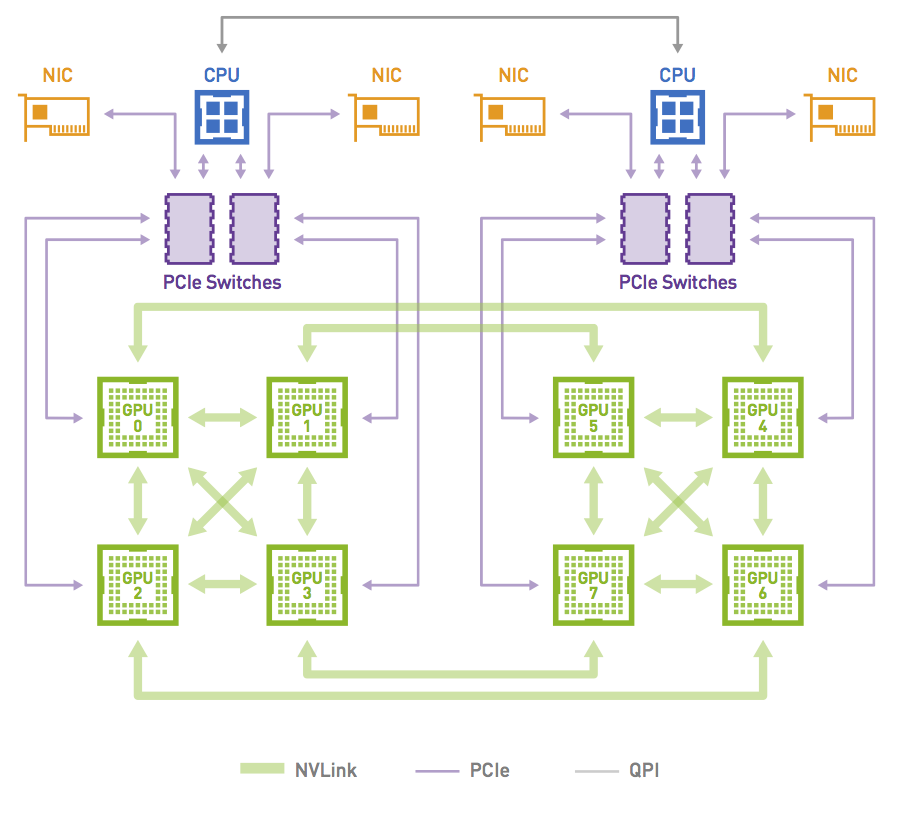
\includegraphics[scale=0.66]{08.MPI_Network/NVLink.png}\\
    PCIe link: 16GB/s\hspace{0.3in}QPI: 25.6GB/s\hspace{0.3in}NVLink: 20GB/s
    \end{center}
\end{frame}

\begin{frame}[fragile]{PCI express}
    \begin{center}
    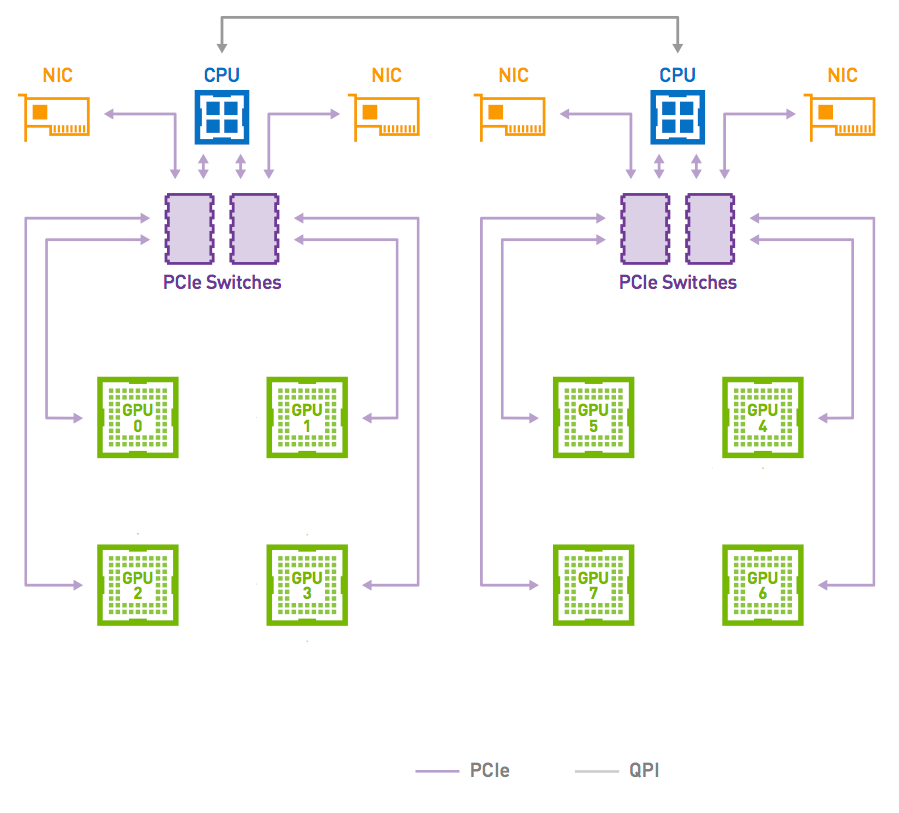
\includegraphics[scale=0.36]{08.MPI_Network/NVLink-pcie.png}
    \begin{itemize}
        \item Connects GPU to CPU socket and GPUs among themselves
        \item Per link: Gen3 1GB/s, Gen4 2GB/s and Gen5 4GB/s
        \item GPUs and CPU sockets connected with 16 links (usually)
        \item Switches with different number of ports
        \item Cuda GPU PeerToPeer enable only on the same socket (root complex)
    \end{itemize}
    \end{center}
\end{frame}

\begin{frame}[fragile]{NVlink}
    \begin{center}
    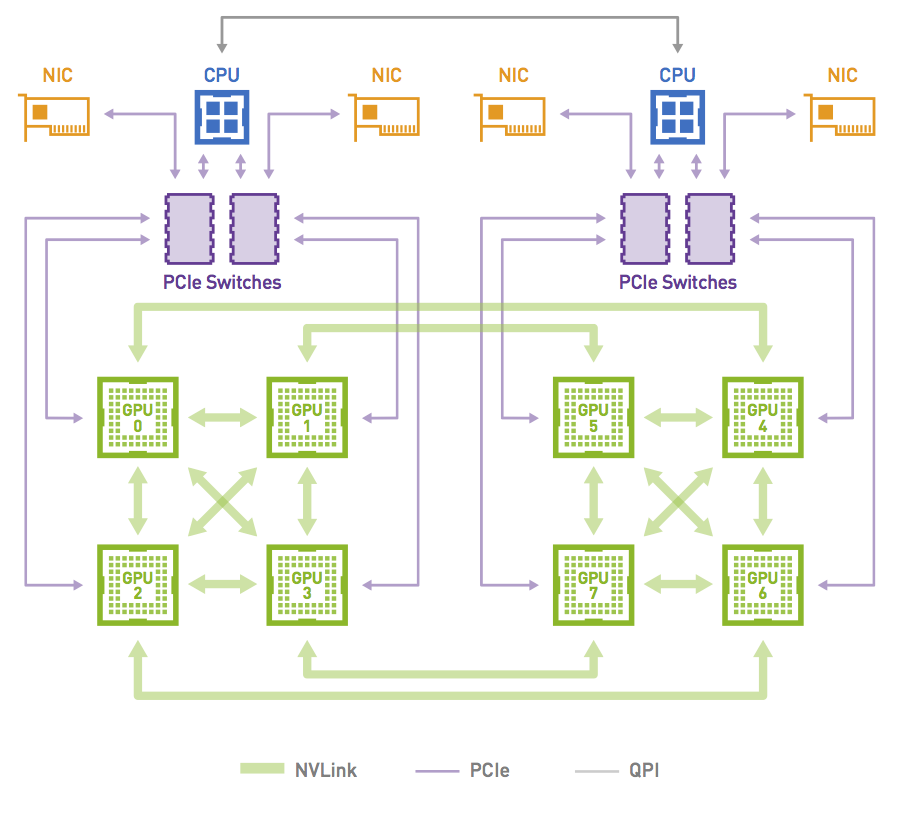
\includegraphics[scale=0.36]{08.MPI_Network/NVLink.png}
    \begin{itemize}
    \item 4 links per GPUs
    \item 20 GB/s per link v1.0 and 25 GB/s for v2.0
    \item Several topology possible
    \item No automatic routing (manually in the application)
    \item NVSwitch fully connects 16 GPUs
    \end{itemize}
    \end{center}
\end{frame}


\begin{frame}[fragile]{HPC network}
    \begin{itemize}
        \item InfiniBand: Fat-tree, FDR 7GB/s, EDR 12.5GB/s, HDR 25GB/s
        \item Cray Aries: Dragonfly, 12GB/s
        \item Others: Intel Omni-Path, 100 Gigabit Ethernet
    \end{itemize}
    OpenFabrics Interfaces (libfabric)
\end{frame}

\cscschapter{Performance of network}

\begin{frame}[fragile]{Bandwidth and latency}
    \begin{itemize}
        \item Bandwidth [GB/s]: the rate of data transfer
        \item Latency [s]: network delay
    \end{itemize}
    Simple performance model: $T = L + M/Bw$
\end{frame}

\begin{frame}[fragile]{Example of performance variability - PCIe}
    \begin{center}
    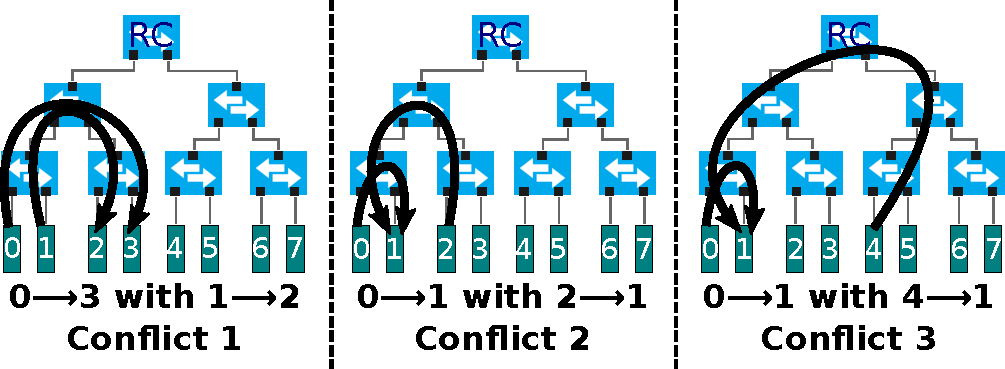
\includegraphics[scale=0.35]{08.MPI_Network/topology_simple_4.pdf}\\
    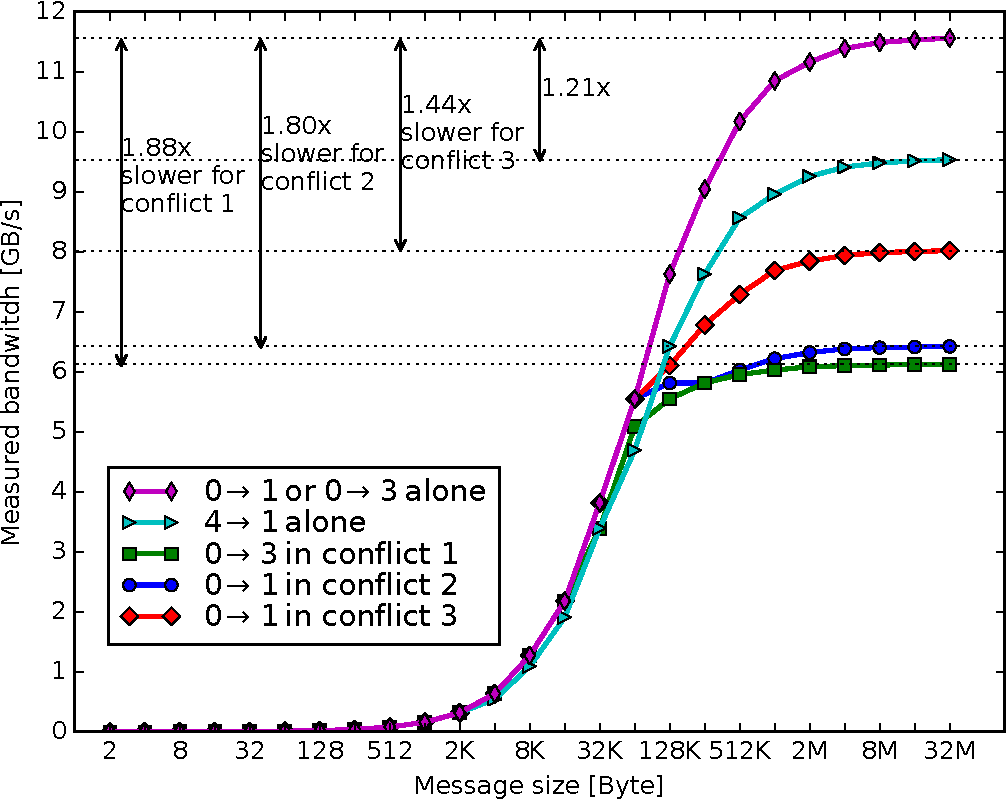
\includegraphics[scale=0.40]{08.MPI_Network/comb_all_plot2.pdf}
    \end{center}
\end{frame}

%\begin{frame}[fragile]{Exercise}
%Bandwidth exercise extended
%\end{frame}

\cscschapter{Communication model and performance}

\begin{frame}[fragile]{MPI with data in device memory}
Use GPUs to parallelize on-node computation
    \begin{itemize}
        \item \ldots and MPI for communication between nodes.
    \end{itemize}
To use with data that is in buffers in GPU memory:
\begin{enumerate}
    \item Allocate buffers in host memory;
    \item Manually copy from device to host memory;
    \item Perform MPI communication with host buffers;
    \item Copy received data from host to device memory.
\end{enumerate}
This approach can be very fast.
\begin{itemize}
    \item Have a CPU thread dedicated to asynchronous host-device and MPI communication
\end{itemize}
\end{frame}

\begin{frame}[fragile]{GPU-aware MPI}
GPU-aware MPI implementations can automatically handle
MPI transactions with pointers to GPU memory
\begin{itemize}
    \item GPUdirect Peer to Peer among GPUs on the same node
    \item GPUdirect RDMA among GPUs on different nodes
    \item MVAPICH, OpenMPI, Cray MPI, \ldots
\end{itemize}
    \begin{blue1block}{How it works}
\begin{itemize}
    \item Each pointer passed to MPI is checked to see if it is in
host or device memory. If not set, MPI assumes that all
pointers are to host memory, and your application will
probably crash with segmentation faults
\item Small messages between GPUs (up to 8 k) are copied
directly with RDMA
\item Larger messages are pipelined via host memory
\end{itemize}
    \end{blue1block}
\end{frame}

%%%%%%%%%%%%%%%%%%%%%%%%%%%%%%%%%%%%%%%%%%%%
\begin{frame}[fragile]{How to use G2G communication}
%%%%%%%%%%%%%%%%%%%%%%%%%%%%%%%%%%%%%%%%%%%%
    \begin{itemize}
        \item Set the environment variable \lst{export MPICH_RDMA_ENABLED_CUDA=1}
        \begin{itemize}
            \item If not set, MPI assumes that all pointers are to host memory, and your application will probably crash with segmentation faults
        \end{itemize}
        \item Experiment with the environment variable \lst{MPICH_G2G_PIPELINE}
        \begin{itemize}
            \item Sets the maximum number of 512 kB message chunks that can be in flight (default 16)
        \end{itemize}
    \end{itemize}

   \begin{code}{MPI with G2G example}
        \begin{lstlisting}[style=boxcudatiny]
MPI_Request srequest, rrequest;
auto send_data = malloc_device<double>(100);
auto recv_data = malloc_device<double>(100);

// call MPI with GPU pointers
MPI_Irecv(recv_data, 100, MPI_DOUBLE, source, tag, MPI_COMM_WORLD, &rrequest);
MPI_Isend(send_data, 100, MPI_DOUBLE, target, tag, MPI_COMM_WORLD, &srequest);
        \end{lstlisting}
   \end{code}

\end{frame}

%%%%%%%%%%%%%%%%%%%%%%%%%%%%%%%%%%%%%%%%%%%%
\begin{frame}[fragile]{Capabilities and Limitations}
%%%%%%%%%%%%%%%%%%%%%%%%%%%%%%%%%%%%%%%%%%%%
    \begin{itemize}
        \item Support for most MPI API calls (point-to-point, collectives, etc)
        \item Robust support for common MPI API calls
        \begin{itemize}
            \item i.e.\ point-to-point operations
        \end{itemize}
        \item No support for user-defined MPI data types
    \end{itemize}
\end{frame}

%%%%%%%%%%%%%%%%%%%%%%%%%%%%%%%%%%%%%%%%%%%%
\begin{frame}[fragile]{Exercise: MPI with G2G}
%%%%%%%%%%%%%%%%%%%%%%%%%%%%%%%%%%%%%%%%%%%%
    \begin{itemize}
        \item 2D stencil with MPI in \lst{08.MPI\_Network/cxx/1.diffusion2d\_mpi.cu}
        \item Implement the G2G version
        \begin{enumerate}
            \item can you observe any performance differences?
        \end{enumerate}
    \end{itemize}

\end{frame}

%%%%%%%%%%%%%%%%%%%%%%%%%%%%%%%%%%%%%%%%%%%%
\begin{frame}[fragile]{Exercises: 2D Diffusion with MPI Results}
%%%%%%%%%%%%%%%%%%%%%%%%%%%%%%%%%%%%%%%%%%%%
    \begin{info}{Time for 10,000 time steps \@ 128$\times$131,072 on P100 GPUs}
       \begin{center}
           \begin{tabular}{ccc}
               \hline
               nodes   &   G2G off & G2G on \\
                \hline
               1       &  5.579    &  5.580 \\
               2       &  3.083    &  2.811 \\
               4       &  1.909    &  1.426 \\
               8       &  1.203    &  0.737 \\
              16       &  0.836    &  0.399 \\
           \end{tabular}
       \end{center}
   \end{info}
\end{frame}

\begin{frame}[fragile]{Communication model and software stack}
    \begin{itemize}
        \item MPI use cuda as a communication back-end
        \item Cuda library is one-sided one rank should know the source and target buffers:\\
        \lst{cudaMemcpy(dst, src, count, kind)}
    \end{itemize}
    What happens when using MPI two-sided?
    \begin{itemize}
        \item Uses IPC to communicate buffer adresses
        \item Lower down the performance
    \end{itemize}
\end{frame}

\begin{frame}[fragile]{Example on halo-exchange}
    \begin{center}
    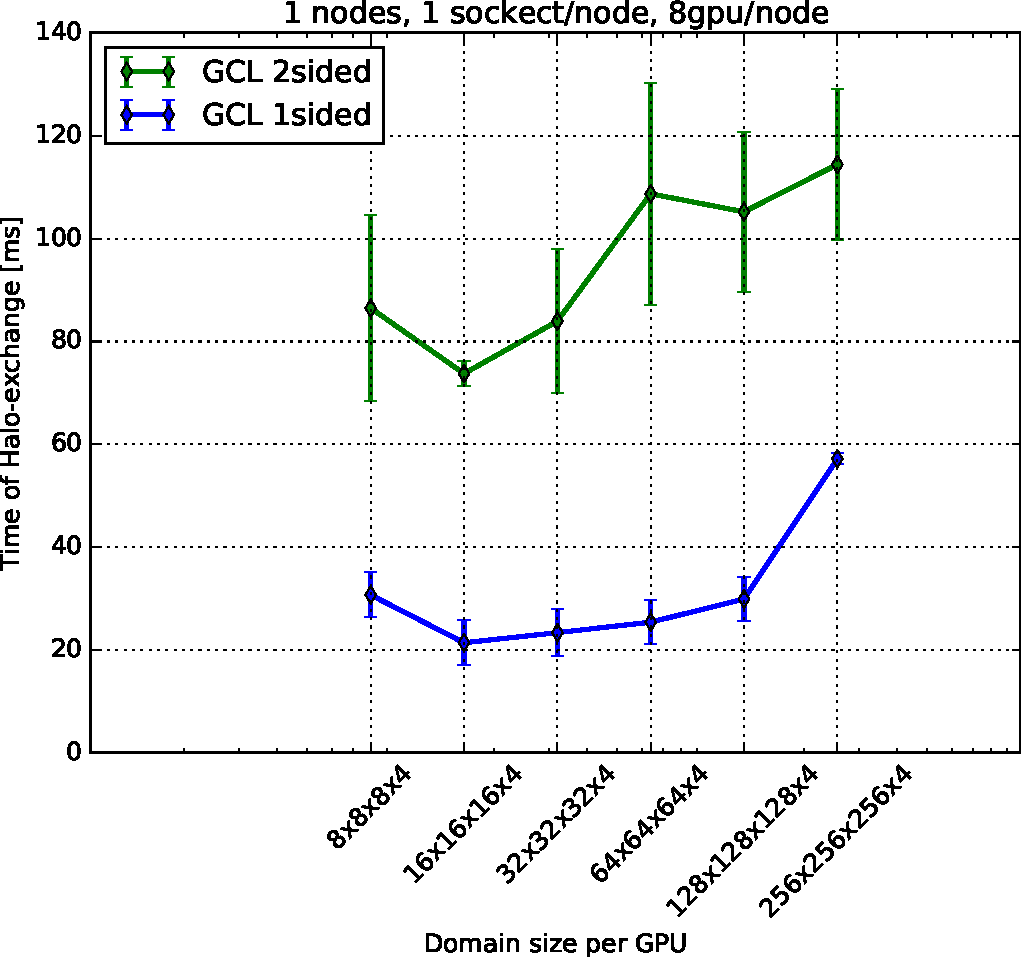
\includegraphics[scale=0.42]{08.MPI_Network/2vs1sided_1n1s8gpu_plot.pdf}\\
    Exchanges 4 halo layers. Exchanges are periodic in all directions.
    \end{center}
\end{frame}


\begin{frame}[fragile]{Misc.}
\begin{itemize}
\item NVidia NCCL: Optimized primitives for collective multi-GPU communication:
all-reduce, all-gather, reduce-scatter, reduce, broadcast
\item OSU (Ohio State University) benchmarks for MPI
\end{itemize}
\end{frame}

% THANK YOU SLIDE
\cscsthankyou{Thank you for your attention.}

\end{document}
